\section{Quantizzazione del campo elettromagnetico}
Abbiamo visto le equazioni per il potenziale elettromagnetico che possono essere riscritte in forma manifestamente covariante introducendo il tensore antisimmetrico $F^{\mu\nu}$.
$$
F^{\mu\nu} = \partial^\mu A^\nu - \partial^\nu A^\mu
$$
Il tensore $F^{\mu\nu}$ è lasciato invariato da una trasformazione di gauge del potenziale
$$
A^\mu \to A'^\mu = A^\mu + \partial^\mu \chi
$$
Infatti
$$
F'^{\mu\nu} = \partial^\mu A'^\nu - \partial^\nu A'^\mu = \partial^\mu A^\nu + \partial^\mu\partial^\nu \chi - (\partial^\nu A^\mu + \partial^\nu\partial^\mu \chi) = F^{\mu\nu}
$$
Le equazioni di Maxwell con le sorgenti sono
$$
\partial_\mu F^{\mu\nu} = J^\nu
$$
Nel vuoto (in assenza di correnti e cariche) diventano
$$
\partial_\mu F^{\mu\nu} = 0 \qquad \partial_\mu\partial^\mu A^\nu + \partial^\nu\partial_\mu A^\mu = 0
$$
Nel gauge di Lorentz ($\partial_\mu F^{\mu\nu}=0$) le equazioni diventano
$$
\partial_\mu\partial^\mu A^\nu = 0 \qquad \Box A^\nu = 0
$$
L'equazione ha una semplice soluzione di onda piana
$$
A^\mu(x) = N \varepsilon^\mu e^{-ik\cdot x}
$$
Nella soluzione $N$ è un fattore di normalizzazione $\varepsilon^\mu$ è il vettore di polarizzazione del potenziale ed infine il quadrivettore $k=(k^0,\mathbf{k})$ con $k^2=0$ è il quadri-momento del fotone. La condizione del gauge di Lorentz diventa.
$$
\partial_\mu A^\mu = 0 \qquad k_\mu \varepsilon^\mu e^{-ik\cdot x} = 0 \qquad k_\mu \varepsilon^\mu = 0
$$
Pertanto delle $4$ componenti di $\varepsilon^\mu$ solo tre sono indipendenti. Tuttavia c'è ancora una ridondanza. $F^{\mu\nu}$ è invariante per l'ulteriore trasformazione ($\partial_\mu A^\mu$ è già uguale a zero). Infatti
$$
A'^\mu = A^\mu + \partial^\mu \tilde{\chi} \text{ con } \tilde{\chi}\quad \text{ che soddisfa l'equazione } \quad\partial_\mu \partial^\mu \tilde{\chi} = 0 \to \tilde{\chi} = i \beta N e^{-ik\cdot x}
$$
Infatti $A'^\mu$ conduce, ovviamente, allo stesso $F^{\mu\nu}$. Inoltre continua a soddisfare il gauge di Lorentz
$$
\partial_\mu A'^\mu = \partial_\mu A^\mu + \partial_\mu \partial^\mu \tilde{\chi} = 0
$$
Questa invarianza si traduce in una ulteriore arbitrarietà di $\varepsilon^\mu$
$$
A'^\mu = N \varepsilon^\mu e^{-ik\cdot x} + N \beta k^\mu e^{-ik\cdot x} = N \varepsilon'^\mu e^{-ik\cdot x} \qquad \varepsilon'^\mu = \varepsilon^\mu + \beta k^\mu
$$
Infatti la condizione di Lorentz risulta ancora rispettata dato che $k_\mu k^\mu=0$
$$
k_\mu \varepsilon'^\mu = k_\mu \varepsilon^\mu + \beta k_\mu k^\mu = k_\mu \varepsilon^\mu + 0 = k_\mu \varepsilon^\mu = 0
$$
Quest'ultima ridondanza deriva dalla massa nulla del fotone: $k_\mu k^\mu=0$. Quest'ultima ridondanza ci permette di ridurre a due i gradi di libertà del campo elettromagnetico. Infatti, data una soluzione $A^\mu=N\varepsilon^\mu e^{-ik\cdot x}$
$$
k = (k^0, \mathbf{k}) \qquad k^0 = |\mathbf{k}| \qquad \varepsilon = (\varepsilon^0, \boldsymbol{\varepsilon}) \qquad k \cdot \varepsilon = 0
$$
Possiamo fare ancora una trasformazione $\varepsilon^\mu\to\varepsilon^\mu+\beta k^\mu$ in modo da annullare la componente temporale $\varepsilon=(0,\boldsymbol{\varepsilon})$. La condizione di Lorentz diventa
$$
k \cdot \varepsilon = 0 \qquad \mathbf{k} \cdot \boldsymbol{\varepsilon} = 0
$$
In pratica si ritorna al gauge di Coulomb e quindi ci sono solo due polarizzazioni indipendenti. Scegliamo una direzione di propagazione lungo l'asse $z$. Le due polarizzazioni possono essere:
\begin{itemize}
    \item Polarizzazione lineare $\boldsymbol{\varepsilon}_1 = (1, 0, 0) \qquad \boldsymbol{\varepsilon}_2 = (0, 1, 0)$
    \item Polarizzazione circolare $\boldsymbol{\varepsilon}_{\lambda=+1} = \frac{1}{\sqrt{2}}(1, i, 0) \qquad \boldsymbol{\varepsilon}_{\lambda=-1} = \frac{1}{\sqrt{2}}(1, -i, 0)$
\end{itemize}
I vettori introdotti soddisfano la relazione 
$$
\boldsymbol{\varepsilon}_\lambda^* \cdot \boldsymbol{\varepsilon}_{\lambda'} = \delta_{\lambda\lambda'} \qquad \lambda, \lambda' = 1, 2
$$
Utilizzando i quadrivettori
$$
\varepsilon^\mu(\lambda) = (0, \boldsymbol{\varepsilon}_\lambda) \qquad \lambda = 1, 2 \qquad \varepsilon_{\mu}^* \varepsilon^\mu_{\lambda'} = - \delta_{\lambda\lambda'}
$$
Ricordiamo che lo sviluppo fatto non è sostanzialmente differente a quello fatto utilizzando il gague di Coulomb. Anche in questo caso la scelta di rendere $\varepsilon^0=0$ non è covariante (funziona in un sistema di riferimento particolare). Tuttavia abbiamo messo in evidenza come la riduzione dei due gradi di libertà dipenda: dalla variazione di gauge e dal fatto che il fotone abbia massa nulla. Utilizzando le onde piane così definite possiamo sviluppare il campo elettromagnetico in integrale di Fourier
$$
A^\mu(x) = \sum_{\lambda=1,2} \int \frac{d^3\mathbf{k}}{(2\pi)^3 \sqrt{2|\mathbf{k}|}} \left( \varepsilon^\mu_{k,\lambda} c_{k,\lambda} e^{-ik\cdot x} + \varepsilon^{\mu *}_{k,\lambda} c^*_{k,\lambda} e^{+ik\cdot x} \right) \qquad 
\lambda = 1,2 \quad c_{\mathbf{k},\lambda}, c^*_{\mathbf{k},\lambda}
$$
La quantizzazione si potrebbe fare promuovendo le ampiezze $c_{\mathbf{k},\lambda}$ e $c^*_{\mathbf{k},\lambda}$ ad operatori di creazione e distruzione e imponendo le regole di commutazione. Tuttavia una tale procedura non è soddisfacente. Non è covariante, vale solo in un dato sistema di riferimento. Non si riesce a derivare dalla quantizzazione canonica del campo elettromagnetico. Vediamo più nel dettaglio la natura delle difficoltà. L'equazione $\Box A^\nu=0$ può essere derivata dalla lagrangiana
$$
\mathcal{L} = -\frac{1}{4} F_{\mu\nu} F^{\mu\nu} \qquad F^{\mu\nu} = \partial^\mu A^\nu - \partial^\nu A^\mu \qquad \mathcal{L} = -\frac{1}{4}(\partial_\mu A_\nu - \partial_\nu A_\mu)(\partial^\mu A^\nu - \partial^\nu A^\mu)
$$
Infatti, dalle equazioni di Eulero-Lagrange
$$
\partial_\mu \left( \frac{\partial\mathcal{L}}{\partial(\partial_\mu A_\nu)} \right) = \frac{\partial\mathcal{L}}{\partial A_\nu} \qquad \frac{\partial\mathcal{L}}{\partial(\partial_\mu A_\nu)} = -(\partial^\mu A^\nu - \partial^\nu A^\mu) \qquad \partial_\mu (\partial^\mu A^\nu - \partial^\nu A^\mu) = 0
$$
$$
\partial_\mu\partial^\mu A^\nu - \partial^\nu\partial_\mu A^\mu = 0 \quad \text{ nel gauge di Lorentz }\quad\partial_\mu A^\mu = 0 \to \Box A^\nu = 0
$$
Per procedere con la quantizzazione occorre calcolare i momenti coniugati evidenziando i termini che contengono $\partial_0 A_\mu$ in $\mathcal{L}$
$$
\pi^\mu = \frac{\partial\mathcal{L}}{\partial(\dot{A}_\mu)} = \frac{\partial\mathcal{L}}{\partial(\partial_0 A_\mu)} \qquad \mathcal{L} \sim -(\partial_0 A_\nu - \partial_\nu A_0)(\partial^0 A^\nu - \partial^\nu A^0)
$$
$$
\pi^\mu = \frac{\partial\mathcal{L}}{\partial(\partial_0 A_\mu)} = -\partial^0 A^\mu + \partial^\mu A^0 \qquad \pi^k = -(\partial^0 A^k - \partial^k A^0) = \partial^k A^0 - \dot{A}^k \quad k=1,2,3
$$
Per $\mu=0$
$$
\pi^0 = \partial^0 A^0 - \partial^0 A^0 = 0
$$
Pertanto la componente $A^0$ non ha un momento coniugato e quindi non si possono imporre regole di commutazione su tutte e $4$ le componenti. Osserviamo che l'equazione dell'onda si ottiene imponendo il gauge di Lorentz. Pertanto la Lagrangiana utilizzata conduce ad una equazione più generale. Si può utilizzare una Lagrangiana diversa che conduca direttamente all'euqazione dell'onda elettromagnetica
$$
\mathcal{L} = -\frac{1}{4} F_{\mu\nu} F^{\mu\nu} \quad \Longrightarrow \quad \mathcal{L} = -\frac{1}{4} F_{\mu\nu} F^{\mu\nu} - \frac{1}{2}(\partial_\mu A^\mu)^2
$$
Ricordiamo la definizione dei momenti coniugati
$$
\pi^\mu = \frac{\partial\mathcal{L}}{\partial(\partial_0 A_\mu)}
$$
Il nuovo pezzo di $\mathcal{L}$ non contiene termini $\partial_0A_\mu$ per $\mu=1,2,3$. I corrispondenti momenti coniugati rimangono invariati
$$
\pi^k = \partial^k A^0 - \dot{A}^k = E^k \qquad k = 1,2,3
$$
Per il momento coniugato $\pi^0$ si trova $\pi^0=-\left(\partial_\mu A^\mu\right)$. Abbiamo trovato $4$ momenti coniugati diversi da zero. Possiamo quindi promuovere campi e momenti coniugati a operatori e imporre le regole di commutazione canoniche
$$
[\hat{A}_\mu(\mathbf{r}, t), \hat{\pi}_\nu(\mathbf{r}', t)] = i g_{\mu\nu} \delta^3(\mathbf{r} - \mathbf{r}')
$$
Il tensore $g^{\mu\nu}$ appare per la natura $4-$vettoriale degli operatori. Ricordiamo la condizione di Lorentz era stata un ingrediente essenziale per ridurre a due il numero di gradi di libertà del sistema. Aspettiamoci pertanto l'apparizione di aspetti non fisici legati ai due gradi di libertà aggiuntivi che sono rimasti nella formulazione. Sviluppiamo ulteriormente il processo di quantizzazione e imponiamo le altre regole di commutazione
$$
[\hat{A}_\mu(\mathbf{r}, t), \hat{A}_\nu(\mathbf{r}', t)] = 0 \qquad [\hat{\pi}_\mu(\mathbf{r}, t), \hat{\pi}_\nu(\mathbf{r}', t)] = 0
$$
Si può dimostrare che le derivate spaziali di $A_\mu$ commutano
$$
[\partial_k \hat{A}_\mu(\mathbf{r}, t), \hat{A}_\nu(\mathbf{r}', t)] = 0 \qquad [\partial_k \hat{A}_\mu(\mathbf{r}, t), \partial_l \hat{A}_\nu(\mathbf{r}', t)] = 0 \qquad k, l = 1, 2, 3
$$
Pertanto la regola di commutazione canonica si riduce a
$$
\pi^k = \partial^k A^0 - \dot{A}^k \qquad [\hat{A}_\mu(\mathbf{r}, t), \hat{\pi}_\nu(\mathbf{r}', t)] = [\hat{A}_\mu(\mathbf{r}, t), \dot{\hat{A}}_\nu(\mathbf{r}', t)] = i g_{\mu\nu} \delta^3(\mathbf{r} - \mathbf{r}')
$$
Confrontandola con quella del campo di Klein-Gordon reale
$$
[\hat{\phi}(\mathbf{r}, t), \dot{\hat{\phi}}(\mathbf{r}', t)] = i \delta^3(\mathbf{r} - \mathbf{r}')
$$
Osserviamo che le regole di commutazione per $A_0$ hanno il segno diverso da quelle di un campo scalare (ad es. il campo di Klein-Gordon)
$$
[\hat{A}_0(\mathbf{r}, t), \dot{\hat{A}}_0(\mathbf{r}', t)] = -i g_{00} \delta^3(\mathbf{r} - \mathbf{r}')
$$
Vedremo tra poco che il segno differente è di fondamentale importanza. Possiamo a questo punto sviluppare il campo elettromagnetico
$$
\hat{A}^\mu(x) = \sum_{\lambda=0}^3 \int \frac{d^3\mathbf{k}}{(2\pi)^3 \sqrt{2|\mathbf{k}|}} \left( \varepsilon^\mu_{k,\lambda} \hat{\alpha}_{k,\lambda} e^{-ik\cdot x} + \varepsilon^{\mu *}_{k,\lambda} \hat{\alpha}_{k,\lambda}^\dagger e^{+ik\cdot x} \right)
$$
NB: $\lambda=0,1,2,3$. A differenza di quanto fatto con il campo classico adesso la somma sugli stati di polarizzazione è adesso estesa a tutti e $4$ gli stati. Costruiremo esplicitamente i $4-$vettori $\varepsilon_{\mu\mathbf{k},\lambda}$ per un arbitrario $k=(|k|, \mathbf{k})$ per il momento è sufficiente dire che
$$
k_\mu \varepsilon^{\mu}_{k,1} = k_\mu \varepsilon^{\mu}_{k,2} = 0 \qquad k_\mu \varepsilon^{\mu}_{k,0} = -k_\mu \varepsilon^{\mu}_{k,3} \qquad \varepsilon_{\mu, k, \lambda} \varepsilon^{\mu}_{k, \lambda'} = g_{\lambda\lambda'}
$$
Dalle regole di commutazione dei campi $A_\mu$ si derivano le regole per gli operatori di creazione e distruzione
$$
[\hat{\alpha}_{k,\lambda}, \hat{\alpha}_{k',\lambda'}^\dagger] = -g_{\lambda\lambda'} (2\pi)^3 \delta^3(\mathbf{k} - \mathbf{k}')
$$
Ancora una volta notiamo la presenza del segno meno per $\lambda=\lambda'=0$. La sua presenza causa un grave problema di autoconsistenza della teoria. Vedremo infatti, nella prossima diapositiva, che compaiono degli stati con norma negativa priva di significato fisico. Come nel caso dei campi di Klein-Gordon e di Dirac utilizziamo gli opeatori di creazione per costruire gli stati a partire dal vuoto
$$
|k, \lambda\rangle = \hat{\alpha}_{k, \lambda}^\dagger |0\rangle
$$
Calcoliamo la norma dello stato
$$
\langle k, \lambda | k', \lambda' \rangle = \langle 0 | \hat{\alpha}_{k, \lambda} \hat{\alpha}_{k', \lambda'}^\dagger |0\rangle = \langle 0 | \cancel{\hat{\alpha}_{k', \lambda'}^\dagger \hat{\alpha}_{k, \lambda}} - g_{\lambda\lambda'} (2\pi)^3 \delta^3(\mathbf{k} - \mathbf{k}') |0\rangle
$$
$$
\langle k, \lambda | k', \lambda' \rangle = -g_{\lambda\lambda'} (2\pi)^3 \delta^3(\mathbf{k} - \mathbf{k}')
$$
Per $\lambda=0$ gli stati hanno norma negativa 
$$
\langle k, 0 | k', 0 \rangle = - (2\pi)^3 \delta^3(\mathbf{k} - \mathbf{k}')
$$
Un tale risultato è inaccettabile; conduce a probabilità negative. Un'altra conseguenza grave è che l'Hamiltoniana non è più definita positiva. In modo analogo a quanto fatto per il campo scalare reale si può calcolare l'Hamiltoniana del campo elettromagnetico
$$
H = \frac{1}{(2\pi)^3} \int d^3k (\hat{\alpha}_{k,1}^\dagger \hat{\alpha}_{k,1} + \hat{\alpha}_{k,2}^\dagger \hat{\alpha}_{k,2} + \hat{\alpha}_{k,3}^\dagger \hat{\alpha}_{k,3} - \hat{\alpha}_{k,0}^\dagger \hat{\alpha}_{k,0}) \omega_k
$$
Inoltre è evidente che la componente temporale $0$ può dare un contributo negativo all'energia. Nel caso classico la scelta del gauge di Lorentz aveva lasciato due gradi di libertà eliminando gli stati con polarizzazione time-like e longitudinali. Abbiamo visto che non possiamo richiedere la relazione operatoriale $\partial_\mu \hat{A}^\mu=0$ senza incorrere in problemi di autoconsistenza. Gupta e Bleuler proposero di imporre una condizione più debole. Definiamo
$$
\hat{A}^{\mu(+)}(x) = \sum_{\lambda=0}^3 \int \frac{\varepsilon^\mu_{k,\lambda} \hat{\alpha}_{k,\lambda} e^{-ik\cdot x}}{(2\pi)^3 \sqrt{2|\mathbf{k}|}} d^3\mathbf{k} \qquad\hat{A}^{\mu(-)}(x) = \sum_{\lambda=0}^3 \int \frac{\varepsilon^{\mu*}_{k,\lambda} \hat{\alpha}_{k,\lambda}^\dagger e^{+ik\cdot x}}{(2\pi)^3 \sqrt{2|\mathbf{k}|}} d^3\mathbf{k}
$$
La condizione proposta è di restringere gli stati fisici $|\Psi\rangle$ dello spazio di Fock solo a quelli che soddisfano la condizione
$$
\langle \Psi | \partial_\mu \hat{A}^\mu | \Psi \rangle = \langle \Psi | \partial_\mu \hat{A}^{\mu(+)} + \partial_\mu \hat{A}^{\mu(-)} | \Psi \rangle = 0
$$
Equivalente a 
$$
\partial_\mu \hat{A}^{\mu(+)} | \Psi \rangle = 0 \qquad \langle \Psi | \partial_\mu \hat{A}^{\mu(-)} = 0
$$
Per comprendere le implicazioni di questa condizione sviluppiamo la prima relazione
$$
\partial_\mu \hat{A}^{\mu(+)} | \Psi \rangle = \sum_{\lambda=0}^3 \int \frac{k_\mu \varepsilon^\mu_{k,\lambda} \hat{\alpha}_{k,\lambda} e^{-ik\cdot x}}{(2\pi)^3 \sqrt{2|\mathbf{k}|}} d^3\mathbf{k} | \Psi \rangle
$$
Esaminiamo l'integrando: abbiamo visto che per 
$$
\lambda=1,2 \qquad k_\mu \varepsilon^\mu_{k,\lambda} = 0 \qquad \lambda=0,3 \qquad k_\mu \varepsilon^\mu_{k,0} = -k_\mu \varepsilon^\mu_{k,3}
$$
Pertanto 
$$
\sum_{\lambda=0}^3 k_\mu \varepsilon^\mu_{k,\lambda} \hat{\alpha}_{k,\lambda} |\Psi\rangle = (k_\mu \varepsilon^\mu_{k,1} \hat{\alpha}_{k,1} + k_\mu \varepsilon^\mu_{k,2} \hat{\alpha}_{k,2}) |\Psi\rangle + (k_\mu \varepsilon^\mu_{k,0} \hat{\alpha}_{k,0} + k_\mu \varepsilon^\mu_{k,3} \hat{\alpha}_{k,3}) |\Psi\rangle =
$$
$$
= (k_\mu \varepsilon^\mu_{k,0} + k_\mu \varepsilon^\mu_{k,3}) |\Psi\rangle = k_\mu \varepsilon^\mu_{k,0} (\hat{\alpha}_{k,0} - \hat{\alpha}_{k,3}) |\Psi\rangle = 0
$$
Pertanto la condizione di Gupta e Bleuler implica che $(\hat{\alpha}_{k,0} - \hat{\alpha}_{k,3}) |\Psi\rangle = 0$. Vediamo adesso l'effetto di questa condizione sul valore di aspettazione dell'Hamiltoniana in uno stato $|\Psi\rangle$
$$
\langle \Psi | \hat{H} | \Psi \rangle = \frac{1}{(2\pi)^3} \int d^3k \langle \Psi | (\hat{\alpha}_{k,1}^\dagger \hat{\alpha}_{k,1} + \hat{\alpha}_{k,2}^\dagger \hat{\alpha}_{k,2} + \hat{\alpha}_{k,3}^\dagger \hat{\alpha}_{k,3} - \hat{\alpha}_{k,0}^\dagger \hat{\alpha}_{k,0}) \omega_k | \Psi \rangle
$$
Analizziamo i contributo $\lambda=0$ e $\lambda=3$ dell'integrando.
$$
\langle \Psi | (\hat{\alpha}_{k,3}^\dagger \hat{\alpha}_{k,3} - \hat{\alpha}_{k,0}^\dagger \hat{\alpha}_{k,0}) | \Psi \rangle = \langle \Psi | (\hat{\alpha}_{k,0}^\dagger \hat{\alpha}_{k,3} - \hat{\alpha}_{k,0}^\dagger \hat{\alpha}_{k,0}) | \Psi \rangle = \langle \Psi | \hat{\alpha}_{k,0}^\dagger (\hat{\alpha}_{k,3} - \hat{\alpha}_{k,0}) | \Psi \rangle = 0
$$
Pertantoal valore di aspettazione dell'Hamiltoniana contribuiscono solo gli stati con polarizzazione trasversale (gli stati con significato fisico). Per semplicità la trattazione è stata intuitiva e parziale, tuttavia mostra una via per quantizzare il campo elettromagnetico utilizzando il metodo canonico. Applicheremo questi concetti ad alcuni processi di elettrodinamica quantistica. Utilizzeremo la rappresentazione del campo
$$
\hat{A}^\mu(x) = \sum_{\lambda=1,2} \int \frac{d^3\mathbf{k}}{(2\pi)^3 \sqrt{2|\mathbf{k}|}} \left( \varepsilon^\mu_{\mathbf{k},\lambda} \hat{\alpha}_{\mathbf{k},\lambda} e^{-ik\cdot x} + \varepsilon^{\mu *}_{\mathbf{k},\lambda} \hat{\alpha}_{\mathbf{k},\lambda}^\dagger e^{+ik\cdot x} \right)
$$
Osserviamo che la somma sulle polarizzazioni è limitata da $\lambda=1,2$. Gli stati fisici rispettano la condizione di Gupta e Bleuler. Gli operatori $\alpha$ creano stati con polarizzazioni $\lambda=1,2$. Le onde piane dell'onda elettromagnetica sono $\varepsilon_{\mathbf{k},\lambda}^\mu e^{-ik\cdot x}$. Tuttavia questo metodo si può applicare solo all'elettrodinamica. Diventa praticamente impossibile per teorie più complicate ad esempio per i quanti dell'interazione debole $Z^{0}$ e $W^{\pm}$. Si usano tecniche più potenti in particolare l'integrale di cammino (Path Integral) ma non ci addentreremo in questi problemi.
\section{Campi interagenti}
La teoria quantistica dei campi fin qui vista descrive l'evoluzione di particelle libere. Gli operatori numero $\hat{N}_k=a_\mathbf{k}^\dagger a_\mathbf{k}$ commutano con l'Hamiltoniana. Il numero delle particelle presenti in ogni modo rimane costante. Non abbiamo quindi risolto il problema di avere una teoria capace di descrivere un numero di particelle variabile nel tempo. Quindi è necessaria una teoria con campi interagenti. Una trattazione rigorosa di campi interagenti va oltre gli obiettivi di questo corso tuttavia discutiamo brevemente alcuni aspetti. Ritorniamo all'oscillatore quantistico unidimensionale
$$
\hat{H}=\frac{\hat{p}^2}{2m}+\frac{1}{2}m\omega^2\hat{q}^2
$$
L'energia potenziale è una forma quadratica e di solito è un risultato di approssimazioni al primo ordine essenziale per trovare soluzioni algebriche che implica la conservazione del numero di quanti ($N$ commuta con $H$). Per introdurre la possibilità di variazione del numero dei quanti occorre andare oltre l'approssimazione armonica. Introduciamo un termine di terzo grado
$$
\hat{H} = \frac{\hat{p}^2}{2m} + \frac{1}{2}m\omega^2\hat{q}^2 + \lambda\hat{q}^3
$$
Esprimendo l'Hamiltoniano in giunzione degli operatori $a$ e $a^\dagger$
$$
\hat{H} = \frac{1}{2}(\hat{a}^\dagger\hat{a} + \hat{a}\hat{a}^\dagger)\omega + \lambda(\hat{a} + \hat{a}^\dagger)^3 \equiv \hat{H}_0 + \lambda\hat{H}'
$$
Quel cubo significa che ho tre campi e quindi ho effettivamente interazione. Non si può risolvere con i metodi algebrici utilizzati precedentemente ma si può verificare che $N=a^\dagger a$ e $H'$ non commutano (gli autovettori di $H$ hanno un numero variabile di quanti). Non esiste una relazione esatta di questo problema e si ricorre al metodo perturbativo. Si tratta il termine $\lambda H'$ come perturbazione. Si espandono gli autovettori (e autovalori) di $H$ in funzione degli autovettori dell'Hamiltoniana imperturbata $H_0$. Agli atuovettori imperturbati $|r\rangle$ corrispondono gli autovettori perturbati $|\overline{r}\rangle$
$$
\hat{H}|\overline{r}\rangle = \overline{E}_r |\overline{r}\rangle \qquad |\overline{r}\rangle = \sum_n c_{rn} |n\rangle \qquad \hat{H}_0 |n\rangle = E_n^{(0)} |n\rangle
$$
$$
\overline{E}_r = E_r^{(0)} + \lambda E_r^{(1)} + \lambda^2 E_r^{(2)} + \dots
$$
Si trova il seguente risultato
$$
\hat{H}_0 |r\rangle = E_r^{(0)} |r\rangle \quad E_r^{(1)} = \langle r | \hat{H}' | r \rangle \quad E_r^{(2)} = \sum_{r \neq s} \frac{\langle r | \hat{H}' | s \rangle \langle s | \hat{H}' | r \rangle}{E_r^{(0)} - E_s^{(0)}}
$$
La correzione al primo ordine è
$$
\langle r | \hat{H}' | r \rangle = \langle r | (\hat{a} + \hat{a}^\dagger)^3 | r \rangle
$$
Per calcolare la correzone al secondo ordine occorre calcolare elementi di matrice del tipo
$$
\langle r | \hat{H}' | s \rangle = \langle r | (\hat{a} + \hat{a}^\dagger)^3 | s \rangle
$$
Inoltre è facile rendersi conto che il secondo elemento di matrice è diverso da zero anche per $s\not=r$, in particolare per $s=r+3,r+1,r-1,r-3$. Questa semplice discussione mostra che l'introduzione di un termine anarmonico ci impone di considerare processi con un numero di particelle non costante. In particolare allo stato $|r\rangle$ (che ha numero definito di quanti) si sostituisce uno stato sovrapposizione di stati contenenti numeri differenti di quanti di $H_0$.
$$
|\overline{r}\rangle = \sum_n c_{rn} |n\rangle
$$
Nella derivazione della Lagrangiana del campo il termine del potenziale era diventato
$$
\tau \Delta x \left( \frac{q_n - q_{n-1}}{\Delta x} \right)^2 \to \tau \left( \frac{\partial \phi}{\partial x} \right)^2 dx
$$
Prodotto di due campi
$$
\lambda q^3 \to \lambda \phi^3
$$
L'interazione è rappresentata dal prodotto di almeno tre campi. Abbiamo già visto la forma di alcune interazioni (corrente per un potenziale)
$$
M_{fi} = -i \int d^4x j_{em}^\mu(x) A_\mu(x)
$$
Klein-Gordon
$$
j_{em}^\mu = iq [\phi_f^* \partial^\mu \phi_i - (\partial^\mu \phi_f^*) \phi_i]
$$
Dirac
$$
j_{em}^\mu = q \overline{\psi}_f(x) \gamma^\mu \psi_i(x)
$$
Come esempio l'interazione di un fermione con il campo elettromagnetico (vediamo subito la presenza di due campi: $\overline{\psi}$ e $\psi$). Facendo il prodotto di questi due campi con il terzo campo che in questo caso è il campo elettromagnetico
$$
\mathcal{L}_D = \overline{\psi}(i\gamma^\mu\partial_\mu - m)\psi \qquad \mathcal{L}_A = -\frac{1}{4} F^{\mu\nu} F_{\mu\nu} \qquad F_{\mu\nu} = \partial_\mu A_\nu - \partial_\nu A_\mu
$$
$$
\mathcal{L}' = -e\overline{\psi}\gamma^\mu\psi A_\mu \qquad \mathcal{L} = \mathcal{L}_D + \mathcal{L}_A + \mathcal{L}'
$$
Quindi abbiamo una lagrangiana libera di Dirac, una lagrangiana di particella libera del campo elettromagnetico e una lagrangiana di interazione (composta da tre campi).
Notare che è il prodotto di tre campi: $\overline{\psi}, \psi, A_\mu$. Se l'interazione non contiene derivate dei campi i momenti coniugati della teoria interagente non cambiano rispetto a quelli della teoria libera. L'Hamiltoniana è pertanto
$$
\mathcal{H} = \mathcal{H}_D + \mathcal{H}_A + \mathcal{H}' \qquad \mathcal{H}' = -\mathcal{L}'
$$
La Lagrangiana introdotta porta alle seguenti equazioni
$$
i\gamma^\mu\partial_\mu\psi - m\psi = e\gamma^\mu A_\mu\psi \qquad \partial_\nu F^{\mu\nu} = e\overline{\psi}\gamma^\mu\psi
$$
Si tratta di un sistema di equazioni differenziali non lineari. Non si sa risolvere in forma chiusa. Per un tempo fissato è possibile sviluppare i campi in termini di operatori di creazione e distruzione. Ad esempio per $t=0$
$$
\hat{\psi}(\mathbf{r}, 0) = \int \sum_{\sigma=\pm s} \frac{d^3\mathbf{k}}{(2\pi)^3 \sqrt{2E_k}} \left( \hat{a}_{k,\sigma} u_{k,\sigma} e^{+i\mathbf{k}\cdot\mathbf{r}} + \hat{b}_{k,\sigma}^\dagger v_{k,\sigma} e^{-i\mathbf{k}\cdot\mathbf{r}} \right) \qquad\omega_k = \sqrt{\mathbf{k}^2 + m^2}
$$
Purtroppo l'evoluzione di questo sviluppo non può essere fatta come nel caso di campo libero. In particolare non è più vero che il campo ad un successivo tempo $t$ possa essere sviluppato negli stessi operatori di creazione e distruzione
$$
\hat{\psi}(\mathbf{r}, t) \neq \int \sum_{\sigma=\pm s} \frac{d^3\mathbf{k}}{(2\pi)^3 \sqrt{2E_k}} \left( \hat{a}_{k,\sigma} u_{k,\sigma} e^{-i\omega_k t} e^{+i\mathbf{k}\cdot\mathbf{r}} + \hat{b}_{k,\sigma}^\dagger v_{k,\sigma} e^{+i\omega_k t} e^{-i\mathbf{k}\cdot\mathbf{r}} \right)
$$
Questo campo non è soluzione delle equazioni di campo con interazione. Questo infatti è un problema molto complesso che si risolve con metodi perturbativi.
\section{Teoria dello Scattering}
\begin{figure}[h!]
    \centering
    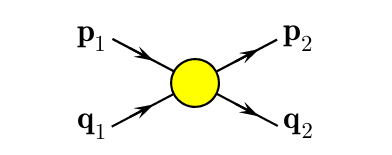
\includegraphics[width=0.7\textwidth]{Lezioni/Lezione 9/sca.png}
    \label{fig:sca}
\end{figure}
Vogliamo adesso vedere come si può descrivere un processo di scattering. Ad esempio lo scattering di $2$ elettroni mediato da interazione elettromagnetica.
$$
e^-+e^-\to e^-+e^-
$$
Si comincia assumento che quando le particelle sono molto distanti l'interazione sia trascurabile e quindi esse possono essere descritte da campi liberi. In particolare, con $a^\dagger(\mathbf{p})$ è l'operatore di creazione degli elettroni, lo stato iniziale è
$$
|\mathbf{p}_1, \mathbf{q}_1\rangle = a^\dagger(\mathbf{p}_1) a^\dagger(\mathbf{q}_1) |0\rangle
$$
Il punto importante è che lo stato $|\mathbf{p}_1,\mathbf{q}_1\rangle$ contiene tutta la storia delle due particelle libere incidenti (non interagenti, libere). Sia nel passato remoto che nel futuro lontano. Stiamo guardando gli stati nella loro rappresentazione di momento. Stiamo fissando il momento. Anche se qui non c'è esplicitamente evoluzione temporale questo rappresenta tutto lo stato evoluto temporalmente. Non è lo stato a $t =-\infty$. Lo stato finale $|\mathbf{p}_2,\mathbf{q}_2\rangle$ non è l'evoluzione libera dello stato $|\mathbf{p}_1,\mathbf{q}_1\rangle$ ma è uno stato differente nel passato e nel futuro. Abbiamo bisogno quindi di un formalismo che mi faccia passare da uno stato iniziale ad uno stato finale differente e capire quale è la probabilità di trovare questo stato. (stati asintotici di particella libera).
\subsection{La matrice S}
Per motivi appena illustrati lo stato iniziale è chiamato stato asintotico $|\rangle_{\text{in}}$
$$
|\mathbf{p}, \mathbf{q}_1\rangle_{\text{in}} = a_{\text{in}}^\dagger(\mathbf{p}_1) a_{\text{in}}^\dagger(\mathbf{q}_1) |0\rangle
$$
Gli stati $|\rangle_{\text{in}}$ formano una base completa dello spazio di Hilbert:
\begin{itemize}
    \item Sono stati di particella NON interagenti
    \item Sono "etichettati" indicando i momenti delle particelle nel passato remoto.
\end{itemize}
Nel passaggio dal passato al futuro le particelle interagiscono e il futuro dello stato che interagisce cambia. Nel futuro l'interazione può portare a stati liberi diversi da quello iniziale. Nel 1943 Heisenberg formulò una teoria dello scattering introducendo un operatore nello spazio di Hilbert: la Matrice S. La matrice S trasforma lo stato asintotico iniziale nello stato finale
$$
S |\mathbf{p}_1,\mathbf{q}_1\rangle_{\text{in}}
$$
Questo stato rappresenta la sovrapposizione di tutti i possibili stati finali (liberi) in cui lo stato iniziale si può trasformare per effetto dell'interazione. Lo stato finale, sovrapposizione di tutte le possibilità. deve avere norma $1$. Ovviamente questo è un operatore complicatissimo e viene costruito a partire da come è fatta l'interazione.
$$
{}_{\text{in}}\langle\mathbf{p}_1,\mathbf{q}_1 | S^\dagger S | \mathbf{p}_1,\mathbf{q}_1 \rangle_{\text{in}} = 1 \qquad S^\dagger S = 1
$$
Quindi la matrice $S$ è unitaria.
\subsection{Teoria dello Scattering}
Noi siamo interessanti al seguente problema. Dato lo stato iniziale
$$
|\mathbf{i}\rangle_\text{in}=|\mathbf{p}_1,\mathbf{q}_1\rangle_{\text{in}}
$$
e calcolare la probabilità di avere uno stato finale
$$
|\mathbf{f}\rangle_\text{in}=|\mathbf{p}_2,\mathbf{q}_2\rangle_{\text{in}}
$$
Stato finale: sono particelle libere che nel futuro hanno momenti $\mathbf{p}_2$ e $\mathbf{q}_2$. Nel passato $|\mathbf{p}_2,\mathbf{q}_2\rangle_{\text{in}}$ rappresenta particelle libere con i momenti indicati mentre nel futuro rappresenterà ancora uno stato di particelle libere con i momenti indicati (evoluzione di particelle libere). Osserviamo che:
\begin{itemize}
    \item Se facciamo variare $|\mathbf{i}\rangle_\text{in}$ fra tutti gli stati della base allora gli stati $S|\mathbf{i}\rangle_\text{in}$ costituiscono un'altra base
    \item Ciò è conseguenza della unitarietà della matrice $S$
    \item Anche gli stati $S|\mathbf{i}\rangle_\text{in}$ sono stati di particelle libere
    \item La matrice $S$ collega stati asintotici ottenuti per $t\to-\infty$ e $t\to+\infty$
    \item Non considera esplicitamente i dettagli dell'interazione posta a $t=0$
\end{itemize}
In conclusione la probabilità cercata è
$$
\wp = | {}_{\text{in}}\langle \mathbf{p}_2, \mathbf{q}_2 | S | \mathbf{p}_1, \mathbf{q}_1 \rangle_{\text{in}} |^2 \qquad \wp = | {}_{\text{in}}\langle f | S | i \rangle_{\text{in}} |^2 = |S_{fi}|^2
$$
\section{Rappresentazione d'Interazione}
Quando si introducono le interazioni non si può più usare la rappresentazione di Heisenberg (campi dipendenti dal tempo - operatori-) perché non si conoscono soluzioni esatte delle equazioni di campo. In particolare non si sa calcolare l'effetto dell'operatore di evoluzione. In questo caso non conosciamo nulla sull'evoluzione temporale e quindi non sappiamo come scriverlo.
$$
\exp[-i\hat{H}(t - t_0)] \qquad H \text{ è l'Hamiltoniano completo}
$$
L'Hamiltoniano completo. Considerando di nuovo l'equazione di Schr\"odinger ($H_0$ è l'Hamiltoniano libero)
$$
\hat{H}\psi_S(\mathbf{r}, t) = i\frac{\partial}{\partial t}\psi_S(\mathbf{r}, t) \qquad \hat{H} = \hat{H}_0 + \hat{H}'
$$
Definiamo, tramite l'operatore evoluzione libero ($t_0=0$) dove il pedice $I$ sta per "interazione" quindi è lo stato in rappresentazione di interazione. Quindi sarebbe l'evoluzione di $\psi_S$ tramite l'hamiltoniano libero.
$$
\psi_I = e^{i\hat{H}_0 t}\psi_S \qquad \psi_S = e^{-i\hat{H}_0 t}\psi_I
$$
Lavorare con questa $\psi_I$ significa che stiamo mettendo un po' di evoluzione temporale che sappiamo (evoluzione libera) che non è interessante perché la conosciamo. Perchè io con la mia teoria perturbativa voglio vedere cosa aggiunge la perturbazione all'interazione libera. Togliamo tutta la parte di interazione libera e ora lo vediamo in maniera pratica. Sostituendo $\psi_S$ nell'equazione di Schr\"odinger
$$
\hat{H}e^{-i\hat{H}_0 t}\psi_I = i\frac{\partial}{\partial t}(e^{-i\hat{H}_0 t}\psi_I) \qquad(\hat{H}_0 + \hat{H}')e^{-i\hat{H}_0 t}\psi_I = \hat{H}_0 e^{-i\hat{H}_0 t}\psi_I + i e^{-i\hat{H}_0 t}\frac{\partial}{\partial t}\psi_I
$$
Moltiplichiamo a sinistra per $\exp{[iH_0t]}$ e poniamo
$$
\hat{H}_I' = e^{i\hat{H}_0 t} \hat{H}' e^{-i\hat{H}_0 t}
$$
$$
(\hat{H}_o + \hat{H}_I')\psi_I = \hat{H}_o \psi_I + i\frac{\partial}{\partial t}\psi_I \qquad \Longrightarrow \qquad \hat{H}_I'\psi_I = i\frac{\partial}{\partial t}\psi_I
$$
Pertanto nella rappresentazione d'interazione l'equazione di evoluzione della funzione d'onda è determinata solo da $H'_I$. Quindi la derivata temporale dello stato in rappresentazione di interazione è determinata solo dal termine di interazione. Questo però mi obbliga a trasformare la $H$ dai campi liberi non dipendenti dal tempo ai campi che hanno dentro tutta l'evoluzione che sarebbe l'evoluzione libera e quindi $H'$. Quindi ora abbiamo un modo formale per scrivere e descrivere la matrice $S$.
\section{Calcolo della Matrice S}
Troviamo una soluzione formale per $\psi_I$
$$
i\frac{\partial}{\partial t}\psi_I = \hat{H}_I'\psi_I
$$
Integrando l'equazione
$$
\int_{-\infty}^t \frac{\partial}{\partial t}\psi_I dt = \psi_I(t) - \psi_I(-\infty) = -i\int_{-\infty}^t \hat{H}_I'\psi_I(t_1) dt_1
$$
$$
\psi_I(t) = \psi_I(-\infty) - i\int_{-\infty}^t \hat{H}_I'\psi_I(t_1) dt_1
$$
Lo stato $\psi(-\infty)$ non è nient'altro che $|i\rangle_\text{in}$ introdotto precedentemente
$$
\psi_I(t) = |i\rangle_{\text{in}} - i\int_{-\infty}^t \hat{H}_I'\psi_I(t_1) dt_1
$$
L'equazione può essere risolta iteraticamente. Infatti al primo ordine, approssimando $\psi_I\approx|i\rangle_\text{in}$ nell'integrando
$$
\psi_I(t) = |i\rangle_{\text{in}} + \int_{-\infty}^t [-i\hat{H}_I'(t_1)] \textcolor{red}{|i\rangle_{\text{in}}} dt_1
$$
Secondo ordine: approssimando nell'integrando $\psi_I(t)$ con la $\psi_I(t)$ del primo ordine
\begin{align*}
\psi_I(t) &= |i\rangle_{\text{in}} + \int_{-\infty}^t [-i\hat{H}_I'(t_1)] |i\rangle_{\text{in}} dt_1 \\
&\quad + \int_{-\infty}^t dt_1 \int_{-\infty}^{t_1} [-i\hat{H}_I'(t_1)] [-i\hat{H}_I'(t_2)] |i\rangle_{\text{in}} dt_2
\end{align*}
Sommando la serie formalmente
$$
\psi_I(t) = \sum_{n=0}^\infty (-i)^n \int_{-\infty}^t dt_1 \int_{-\infty}^{t_1} dt_2 \dots \int_{-\infty}^{t_{n-1}} dt_n [H_I'(t_1) H_I'(t_2) \dots H_I'(t_n)] |i\rangle_{\text{in}}
$$
Ricordiamo che per $t\to+\infty$ abbiamo definito $\psi_I(\infty)=S|i\rangle_\text{in}$ e per confronto troviamo un'espressione per la matrice $S$
$$
\hat{S} = \sum_{n=0}^\infty (-i)^n \int_{-\infty}^{\infty} dt_1 \int_{-\infty}^{t_1} dt_2 \dots \int_{-\infty}^{t_{n-1}} dt_n [\hat{H}_I'(t_1) \hat{H}_I'(t_2) \dots \hat{H}_I'(t_n)]
$$
Nella formula abbiao ribadito la natura operatoriale delle grandezze. Osserviamo che i temi sono ordinati: $t_1 > t_2 > \dots > t_n$. Definiamo l'operatore di ordinamente cronologico $T$
$$
T[\hat{A}(t_1) \hat{A}(t_2)] = \begin{cases} \hat{A}(t_1) \hat{A}(t_2) & t_1 > t_2 \\ \hat{A}(t_2) \hat{A}(t_1) & t_2 > t_1 \end{cases}
$$
Si dimostra che si possono estendere tutti gli integrali a $+\infty$ e si ottiene la serie di Dyson
$$
\hat{S} = \sum_{n=0}^\infty \frac{(-i)^n}{n!} \int dt_1 \int dt_2 \dots \int dt_n T[\hat{H}_I'(t_1) \hat{H}_I'(t_2) \dots \hat{H}_I'(t_n)]
$$
\subsection{Sviluppo perturbativo}
Isoliamo il contributo $n=0$
$$
\hat{S} = \hat{1} + \sum_{n=1}^\infty \frac{(-i)^n}{n!} \int dt_1 \int dt_2 \dots \int dt_n T[\hat{H}_I'(t_1) \hat{H}_I'(t_2) \dots \hat{H}_I'(t_n)]
$$
Notiamo che la matrice $S$ contiene un termine $1$ che tiene conto del fatto che le particelle possono anche non interagire. Si dimostra che gli operatori $H'_I$ sono esprimibili in funzione dei campi liberi $\hat{\psi_I}$. Per il calcolo delle sezioni d'urto o delle larghezze di decadimento occorre calcolare elementi di matrice fra stato iniziale e finale
$$
\langle f | \hat{S} | i \rangle = S_{fi} = \delta_{fi} + \mathcal{A}_{fi} = \delta_{fi} + \langle f | \hat{A} | i \rangle
$$
Abbiamo implicitamente definito l'ampiezza di transizione $A_{fi}$ che vedremo contenere a sua volta una funzione $\delta(p_i-p_f)$ $4-$dimensionale che esprime la conservazione dell'energia e della quantità di moto. Si preferisce fattorizzare anche questo aspetto con una ulteriore matrice
$$
\mathcal{A}_{fi} = (2\pi)^4 \delta(p_i - p_f) \mathfrak{M}_{fi}
$$
\section{Sezione d'urto e vita media}
Nella fisica delle Particelle Elementari si studiano sostanzialmente due fenomeni
\begin{figure}[h!]
    \centering
    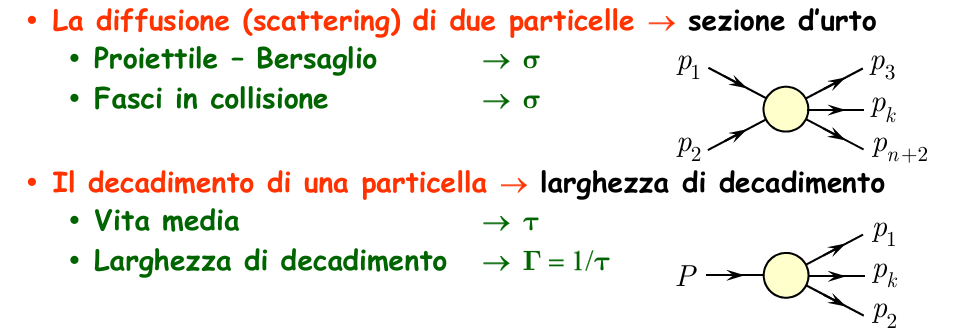
\includegraphics[width=0.8\textwidth]{Lezioni/Lezione 9/lo.png}
    \label{fig:lo}
\end{figure}
Entrambi i processi vengono descritti per mezzo dell'ampiezza invariante di transizione $\mathfrak{M}$
\begin{figure}[h!]
    \centering
    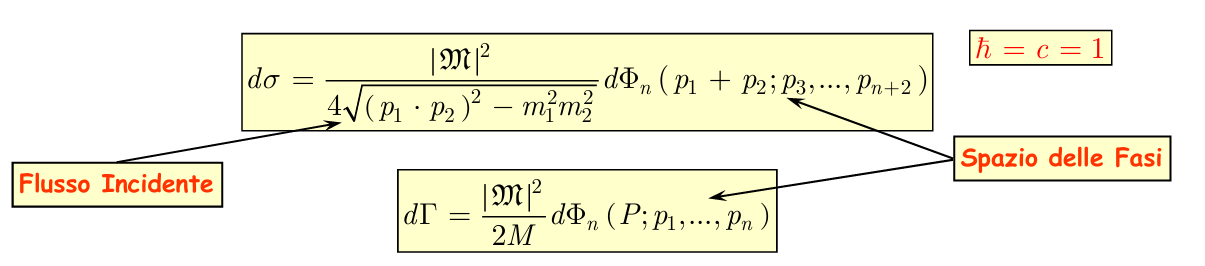
\includegraphics[width=0.8\textwidth]{Lezioni/Lezione 9/li.png}
    \label{fig:li}
\end{figure}